 
%______________________________________________________________________________________________________________________
% @brief    LaTeX2e Resume for Kamil K Wojcicki
\documentclass[margin,line]{resume}
\usepackage[latin1]{inputenc}
\usepackage{graphics}
\usepackage{amsmath,amssymb}
\usepackage{gensymb}
\usepackage{amsthm}
\usepackage{wrapfig,lipsum,booktabs}
\usepackage{caption}
\usepackage{subcaption}
\usepackage{tabulary}
\usepackage{epigraph}
\usepackage{mwe}
\usepackage[autostyle]{csquotes} 
\usepackage{lipsum,lmodern}
\usepackage[skins]{tcolorbox}
\usepackage{pgf,tikz}
\usetikzlibrary{arrows,shapes,backgrounds,fit}
\usetikzlibrary{arrows,automata}

\usepackage{fancyvrb}
\usepackage{listings}
\usepackage{color}
%______________________________________________________________________________________________________________________
\begin{document}
\name{\Large Simon Holmbacka. PhD -- Publications}
\begin{resume}
\begin{picture}(320,0)
\put(320,-160){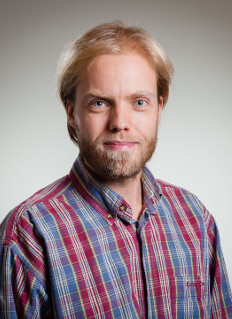
\includegraphics[scale=0.5]{simon.jpg}}
\end{picture}
    %__________________________________________________________________________________________________________________
    % Contact Information
    \section{\mysidestyle Contact\\Information}

    Embedded Systems Laboratory                         	     \vspace{0mm}\\\vspace{0mm}%
    Faculty of Science and Engineering                           \vspace{0mm}\\\vspace{0mm}%
    \AA{}bo Akademi University, Finland			       		\vspace{0mm}\\\vspace{-4.5mm}%
    
\small{
    Tammikalliontie 1			\vspace{0mm}\\\vspace{0mm}%
    20900				\vspace{0mm}\\\vspace{0mm}%
    Turku				\vspace{0mm}\\\vspace{0mm}%
    Finland				\vspace{0mm}\\\vspace{0mm}%
    Tel: +358 50 5310467		\vspace{0mm}\\\vspace{0mm}%
    Email: sholmbac@abo.fi		\vspace{0mm}\\\vspace{-4.5mm}%
    }
\vspace{1.0cm}
\section{\mysidestyle Thesis}    
Simon Holmbacka:
\textit{Energy Aware Software for Many-Core Systems},
Faculty of Science and Engineering,\\ \AA{}bo Akademi University, 2015, Turku, Finland

\section{\mysidestyle Publications -- Journals (5)}
Simon Holmbacka, Dra\v{z}en Lu\v{c}anin , Ilia Pietri, Ivona Brandic, Johan Lilius, Rizos Sakellariou:
\textit{Performance-Based Pricing in Multi-Core Geo-Distributed Cloud Computing}, 
\textsl{IEEE Transactions on Cloud Computing}, IEEE 2016

Simon Holmbacka, J\"{o}rg Keller, Patrick Eitschberger, Johan Lilius:
\textit{Accurate Energy Modeling for Many-Core Static Schedules with Streaming Applications}, 
\textsl{Microprocessors and Microsystems, Elsevier}, 2016

Simon Holmbacka, Erwan Nogues, Maxime Pelcat, S\'{e}bastien Lafond, Daniel Menard, Johan Lilius:
\textit{Energy-Awareness and Performance Management with Parallel Dataflow Applications}, 
\textsl{The Journal Signal Processing Systems. Springer US}, 2015

Jose-Luis Guti\'{e}rrez-Rivas, Simon Holmbacka, Miguel M\'{\i}ndez-Mac\'{\i}as, Wictor Lund, S\'{e}bastien Lafond, Johan Lilius, Javier D\'{\i}az-Alonso:
\textit{Safe Motor Controller in a Mixed-Critical Environment with Runtime Updating Capabilities}, 
\textsl{Journal of Universal Computer Science}, 2015

Simon Holmbacka, Mohammad Fattah, Wictor Lund, Amir-Mohammad Rahmani, S\'{e}bastien Lafond, Johan Lilius:
\textit{A Task Migration Mechanism for Distributed Many-Core Operating Systems}, 
\textsl{The Journal of Supercomputing. Springer US}, 2014 


\section{\mysidestyle Publications -- Proceedings (22)}
Simon Holmbacka, J\"{o}rg Keller
\textit{Workload Type-Aware Scheduling on big.LITTLE Platforms}
\textsl{Proceedings of the 17th International Conference on Algorithms and Architectures on Parallel Processing}, 2017, Helsinki, Finland

J\"{o}rg Keller, Patrick Eitchberger, Simon Holmbacka
\textit{Hardware and Software support for transposition or bit matrices in high-speed encryption}
\textsl{Proceedings of the 17th International Conference on Algorithms and Architectures on Parallel Processing}, 2017, Helsinki, Finland

Simon Holmbacka, Robert M\"{u}ller: 
\textit{epEBench: True Energy Benchmark},
\textsl{25st Euromicro International Conference on Parallel, Distributed and Network-Based Processing}, 2016, St Petersburg, Russia

Hergys Rexha, Simon Holmbacka, S\'{e}bastien Lafond: 
\textit{Core Level Utilization for Achieving Energy Efficiency in Heterogeneous Systems},
\textsl{25st Euromicro International Conference on Parallel, Distributed and Network-Based Processing}, 2016, St Petersburg, Russia

Georgios Georgakarakos, Simon Holmbacka and Johan Lilius
\textit{Analysis on Scalability and Energy Efficiency of HEVC Decoding Using Task-Based Programming Model}
\textsl{The 2016 Conference on Design \& Architectures for Signal \& Image Processing, 2016, Rennes, France}

Enida Sheme, Neki Frash\"{e}ri, Simon Holmbacka, S\'{e}bastien Lafond, Dra\v{z}en Lu\v{c}anin 
\textit{Datacenters Powered by Renewable Energy: A Case Study for 60 Degrees Latitude North}
\textsl{Seventh symposium on green networking and computing (SGCN 2016)},2016, Split, Croatia

Simon Holmbacka, J\"{o}rg Keller, Patrick Eitschberger, Johan Lilius:
\textit{Accurate Energy Modelling for Many-Core Static Schedules}
\textsl{Proceedings of the 23rd International Euromicro Conference on Parallel, Distributed and Network-based Processing}, 2015, Turku, Finland
\clearpage

Simon Holmbacka, Johan Lilius: 
\textit{Fitness: A Metric Describing the Efficiency of Microarchitectual Utilization},
\textsl{Eight Nordic Workshop on Multicore Computing}, 2015, Copenhagen, Denmark

Simon Holmbacka, S\'{e}bastien Lafond, Johan Lilius:
\textit{Performance Monitor Based Power Management for big.LITTLE Platforms}
\textsl{HiPEAC Workshop on Energy Efficiency with Heterogeneous Computing}, 2015, Amsterdam, Netherlands

Simon Holmbacka, Erwan Nogues, Maxime Pelcat, S\'{e}bastien Lafond, Johan Lilius:
\textit{Energy Efficiency and Performance Management of Parallel Dataflow Applications} [\textbf{BEST PAPER}]
\textsl{The 2014 Conference on Design \& Architectures for Signal \& Image Processing}, 2014, Madrid, Spain

Erwan Nogues, Simon Holmbacka, Maxime Pelcat, Daniel Menard, Johan Lilius:
\textit{Power-Aware HEVC Decoding with Tunable Image Quality}
\textsl{2014 IEEE Workshop on Signal Processing Systems}, 2014, Belfast, UK

Simon Holmbacka, Johan Lilius: 
\textit{Evaluation of CPU Hotplug Latency on Multi-Core ARM Chips},
\textsl{Seventh Swedish Workshop on Multicore Computing}, 2014, Lund, Sweden 

Fredric H\"{a}llis, Simon Holmbacka, Wictor Lund, Robert Slotte, S\'{e}bastien Lafond and Johan Lilius:
\textit{Thermal Influence on the Energy Efficiency of Workload Consolidation in Many-Core Architecture}, 
\textsl{Proceedings of the 24th Tyrrhenian International Workshop on Digital Communications}, 2013, Genoa, Italy 

Simon Holmbacka, Wictor Lund, S\'{e}bastien Lafond, Johan Lilius: 
\textit{Lightweight Framework for Runtime Updating of C-Based Software in Embedded Systems},
\textsl{5th Workshop on Hot Topics in Software Upgrades}, 2013, San Jose, US

Simon Holmbacka, Wictor Lund, S\'{e}bastien Lafond, Johan Lilius: 
\textit{QoS Manager for Energy Efficient Many-Core Operating Systems},
\textsl{21st Euromicro International Conference on Parallel, Distributed and Network-Based Processing}, 2013, Belfast, UK

Simon Holmbacka, Dag \AA{}gren, S\'{e}bastien Lafond, Johan Lilius: 
\textit{Task Migration for Dynamic Power and Performance Characteristics on Many-Core Distributed Operating Systems},
\textsl{21st Euromicro International Conference on Parallel, Distributed and Network-Based Processing}, 2013, Belfast, UK

Simon Holmbacka, S\'{e}bastien Lafond, Johan Lilius: 
\textit{Power Optimized Many-Cores with User Centric Notion of Parallelism},
\textsl{Sixth Swedish Workshop on Multicore Computing}, 2013, Halmstad, Sweden
  
Simon Holmbacka, S\'{e}bastien Lafond, Johan Lilius: 
\textit{Towards Increasing Energy Scalability in Many-Core Systems}, 
\textsl{1st ASPLOS Doctoral Workshop}, 2012, London, UK

Simon Holmbacka, S\'{e}bastien Lafond, Johan Lilius: 
\textit{A PID-Controlled Power Manager for Energy Efficient Web Clusters}, 
\textsl{International Conference on Cloud and Green Computing}, 2011, Sydney, Australia 

Simon Holmbacka, S\'{e}bastien Lafond, Johan Lilius: 
\textit{Power Proportional Characteristics of an Energy Manager for Web Clusters}, 
\textsl{11:th International Conference on Embedded Computer Systems: Architctures, Modeling and Simulation}, 2011, Samos, Greece

Simon Holmbacka, Jens Smeds, S\'{e}bastien Lafond, Johan Lilius:
\textit{System Level Power Management for Many-Core Systems},
\textsl{uPM2SoC workshop, DATE '11 Conference}, 2011, Grenoble, France

Simon Holmbacka, S\'{e}bastien Lafond, Johan Lilius: 
\textit{Generic QoS Manager for Many-Core Service-Based Operating Systems}, 
\textsl{Fourth Swedish Workshop on Multicore Computing}, 2011, Link\"{o}ping Sweden

\section{\mysidestyle Publications -- Non-peer-reviewed}
Simon Holmbacka Fredric H\"{a}llis, Wictor Lund, S\'{e}bastien Lafond and Johan Lilius:
\textit{Energy and Power Management, Measurement and Analysis for Multi-Core Processors} 
\textsl{TUCS Technical Reports 1117}, 2014, Turku Centre for Computer Science 

\section{\mysidestyle Registered Inventions}
Simon Holmbacka (100\%):
\textit{Power management with performance monitoring for computer systems}\\Coordinator: Olle Lagerroos, June 2015, \AA{}bo Akademi University
\clearpage
\section{\mysidestyle Referees} 

\begin{tabular}{@{}p{4.2cm}p{6cm}p{5cm}}
\textbf{Prof. Johan Lilius}       &  \textbf{Prof. J\"{o}rg Keller}	&  \textbf{Jonas Kronlund}                   \\
Professor                               &  Professor & Business Design Lead                       \\
\AA{}bo Akademi University                     &  Fernuniversit\"{a}t in Hagen   &   Elisa Oyj                 \\
Turku Finland			           &  Hagen Germany        & Helsinki Finland\\
phone: \textsl{available on request}    &  phone: \textsl{available on request}  &  phone: \textsl{available on request}      \\
e-mail: \textsl{johan.lilius@abo.fi}   &  e-mail: \textsl{joerg.keller@fernuni-hagen.de}  &  e-mail: \textsl{jonas.kronlund@elisa.fi}   \\
\vspace{0.5cm}
\textbf{Prof. Juha Plosila} & &\\
Professor & &\\
University of Turku & &\\
Turku Finland & &\\
phone: \textsl{available on request} & &\\
e-mail: \textsl{juplos@utu.fi} & &\\
\end{tabular}



%______________________________________________________________________________________________________________________

\include{ecourse}

\end{resume}
\end{document}


%______________________________________________________________________________________________________________________
% EOF

